\chapter[Results and Discussions]{Results and Discussions}
\label{ch5}

In this chapter, the results and discussions regarding delamination identification in CFRP plates are presented. 
Accordingly, to verify the developed DL models, I evaluated them on \(95\) unseen numerical test cases and further on experimental test cases.
Moreover, I have selected four numerical test cases to present. 
The selected four numerical cases were chosen to represent the random distribution of delamination locations.
%Figure~\ref{numerical_cases} shows the selected numerical test cases that are evaluated and further presented will the developed models
%
%\begin{figure} [ht!]
%	\centering
%	%%%%%%%%%%%%%%%%%%%%%%%%%%%%%%%%%%%%%%%%%%%%%%%%%%%%%%%%%%%%%%%%%%%%%%%%%%%%
%	%%%%% case 448
%	%%%%%%%%%%%%%%%%%%%%%%%%%%%%%%%%%%%%%%%%%%%%%%%%%%%%%%%%%%%%%%%%%%%%%%%%%%%%
%	\begin{subfigure}[b]{.48\textwidth}
%		\centering
%		\includegraphics[width=5cm]{Figures/Chapter_5/RMS_flat_shell_Vz_448_500x500bottom.png}
%		\caption{First RMS case}
%		\label{fig:RMS_bottom_448}
%	\end{subfigure}
%	\hfill
%	\begin{subfigure}[b]{0.48\textwidth}
%		\centering
%		\includegraphics[width=5cm]{Figures/Chapter_5/m1_rand_single_delam_448.png}
%		\caption{}
%		\label{fig:GT_case_448}
%	\end{subfigure}	
%	\par\medskip
%	%%%%%%%%%%%%%%%%%%%%%%%%%%%%%%%%%%%%%%%%%%%%%%%%%%%%%%%%%%%%%%%%%%%%%%%%%%%%
%	%%%%% case 456
%	%%%%%%%%%%%%%%%%%%%%%%%%%%%%%%%%%%%%%%%%%%%%%%%%%%%%%%%%%%%%%%%%%%%%%%%%%%%%
%	\begin{subfigure}[b]{.48\textwidth}
%		\centering
%		\includegraphics[width=5cm]{Figures/Chapter_5/RMS_flat_shell_Vz_456_500x500bottom.png}
%		\caption{Second RMS case}
%		\label{fig:RMS_bottom_456}
%	\end{subfigure}
%	\hfill
%	\begin{subfigure}[b]{0.48\textwidth}
%		\centering
%		\includegraphics[width=5cm]{Figures/Chapter_5/m1_rand_single_delam_456.png}
%		\caption{}
%		\label{fig:GT_case_456}
%	\end{subfigure}	
%	\hfill
%	\par\medskip
%	%%%%%%%%%%%%%%%%%%%%%%%%%%%%%%%%%%%%%%%%%%%%%%%%%%%%%%%%%%%%%%%%%%%%%%%%%%%%
%	%%%%% case 438
%	%%%%%%%%%%%%%%%%%%%%%%%%%%%%%%%%%%%%%%%%%%%%%%%%%%%%%%%%%%%%%%%%%%%%%%%%%%%%
%	\begin{subfigure}[b]{.48\textwidth}
%		\centering
%		\includegraphics[width=5cm]{Figures/Chapter_5/RMS_flat_shell_Vz_438_500x500bottom.png}
%		\caption{Second RMS case}
%		\label{fig:RMS_bottom_438}
%	\end{subfigure}
%	\hfill
%	\begin{subfigure}[b]{0.48\textwidth}
%		\centering
%		\includegraphics[width=5cm]{Figures/Chapter_5/m1_rand_single_delam_438.png}
%		\caption{}
%		\label{fig:GT_case_438}
%	\end{subfigure}	
%	\par\medskip
%	%%%%%%%%%%%%%%%%%%%%%%%%%%%%%%%%%%%%%%%%%%%%%%%%%%%%%%%%%%%%%%%%%%%%%%%%%%%%
%	%%%%% case 397
%	%%%%%%%%%%%%%%%%%%%%%%%%%%%%%%%%%%%%%%%%%%%%%%%%%%%%%%%%%%%%%%%%%%%%%%%%%%%%
%	\begin{subfigure}[b]{.48\textwidth}
%		\centering
%		\includegraphics[width=5cm]{Figures/Chapter_5/RMS_flat_shell_Vz_397_500x500bottom.png}
%		\caption{Second RMS case}
%		\label{fig:RMS_bottom_397}
%	\end{subfigure}
%	\hfill
%	\begin{subfigure}[b]{0.48\textwidth}
%		\centering
%		\includegraphics[width=5cm]{Figures/Chapter_5/m1_rand_single_delam_397.png}
%		\caption{}
%		\label{fig:GT_case_397}
%	\end{subfigure}	
%	\hfill
%	\par\medskip	
%	\caption{Four selected numerical cases}
%	\label{numerical_cases}
%\end{figure} 
%%%%%%%%%%%%%%%%%%%%%%%%%%%%%%%%%%%%%%%%%%%%%%%%%%%%%%%%%%%%%%%%%%%%%%%%%%%%%%%%

Furthermore, I have applied the super-resolution image reconstruction technique to LR full wavefield animations for both the numerical test cases and the experimental case. 
Then, I applied the AE-ConvLSTM model to the reconstructed frames in order to identify the delamination.

Accordingly, to evaluate the performance of the proposed models, the intersection over union \(IoU\) (Jaccard index) was applied as the accuracy metric.
\(IoU\) is estimated by determining the intersection area between the ground truth and the predicted output.
Furthermore, we have two output classes (damaged and undamaged). 
The \(IoU\) was calculated for the damaged class only.
The illustration of the IoU metric is presented in Fig.~\ref{fig:iou} where Eqn.~(\ref{eqn:iou}) defines the \(IoU\) metric:
%%%%%%%%%%%%%%%%%%%%%%%%%%%%%%%%%%%%%%%%%%%%%%%%%%%%%%%%%%%%%%%%%%%%%%%%%%%%%%%%
\begin{figure} [h!]
	\begin{center}
		\includegraphics[scale=.75]{Figures/Chapter_5/IoU_figure.png}
	\end{center}
	\caption{Intersection over union.} 
	\label{fig:iou}
\end{figure}
%%%%%%%%%%%%%%%%%%%%%%%%%%%%%%%%%%%%%%%%%%%%%%%%%%%%%%%%%%%%%%%%%%%%%%%%%%%%%%%%
\begin{equation}
	\textup{IoU}=\frac{Intersection}{Union}=\frac{\hat{Y} \cap Y}{\hat{Y} \cup Y},
	\label{eqn:iou}
\end{equation}
%%%%%%%%%%%%%%%%%%%%%%%%%%%%%%%%%%%%%%%%%%%%%%%%%%%%%%%%%%%%%%%%%%%%%%%%%%%%%%%%
where \(\hat{Y}\) is the predicted output, and \(Y\) is the ground truth (label).

Additionally, the percentage area error $\epsilon$ depicted in Eqn.~(\ref{eqn:mean_size_error}) was utilised to evaluate the performance of the FCN models and the Autoencoder ConvLSTM model:
\begin{equation}
	\epsilon=\frac{|A-\hat{A}|}{A} \times 100\%,
	\label{eqn:mean_size_error}
\end{equation}
where \(A\) and \(\hat{A}\) refer to the area in mm\textsuperscript{2} of the damage class in the ground truth and the predicted output, respectively.
Such a metric can indicate how close the area of the predicted delamination is to the ground truth.
Accordingly, the lower the value of $\epsilon$, the higher the accuracy of the identified damage. 

Two metrics are utilised for evaluating the DLSR model developed to perform super-resolution image reconstruction of the full wavefield.
The first metric is the peak signal-to-noise ratio (PSNR), which refers to the maximum possible power of a signal and the power of the distorting noise that affects the quality of its representation.
Equation~(\ref{PSNR}) depicts the mathematical representation of the PSNR:
\begin{equation}
	PSNR=20\log_{10}\left(\frac{R}{\sqrt{MSE}}\right),
	\label{PSNR}
\end{equation}
where \(R\) represents the maximum fluctuation value that exists in the input image, and its equal to \(255\), as I used an 8-bit unsigned integer data type.
\(MSE\) refers to the mean square error between the predicted output and the corresponding ground truth (see Eqn.~\ref{mse}).

The second utilised metric is the Pearson correlation coefficient that measures the linear relationship between two variable matrices \textbf{\(X\)} (represents the ground truth values) and \textbf{\(Y\)} (represents the predicted values), and its value is between -1 and 1, where:
\begin{itemize}
	\item -1 represents a perfect negative linear correlation,
	\item 0 represents no linear correlation,
	\item 1 represents a perfect positive linear correlation.
\end{itemize}
Equation~\ref{Pearson} depicts the mathematical formula to calculate Pearson CC commonly denoted as \(r_{xy}\):
\begin{equation}
	r_{xy} = \frac{\sum_{i=1}^{n}(x_i - \bar{x})(y_i-\bar{y})}{\sqrt{\sum_{i=1}^{n}(x_i - \bar{x})^2}\sqrt{\sum_{i=1}^{n}(y_i - \bar{y})^2}},
	\label{Pearson}
\end{equation}
where \(n\) is the number of sample points, \(x_i\), \(y_i\) are the individual value points representing the ground truth and predicted values, respectively, and \(\bar{x}\) is the mean value of the sample, analogously to \(\bar{y}\).


In the following, I will present and discuss the results of the developed CNN classifier models in section~\ref{sec51}. 
In section~\ref{sec52}, the results of the five developed FCN models will be presented and discussed.
Accordingly, a comparison between the developed FCN models will be made.
In section~\ref{sec53}, the results and discussion regarding the developed AE-ConvLSTM model are presented.
Finally, in section~\ref{sec54}, I will present the results of applying the developed DLSR model to numerical cases to identify the damage in the reconstructed frames.
Furthermore, I will apply the DLSR model to an experimental scenario to identify the delamination.
%% INCLUDE SECTIONS ////////////////////////////////////////////////////////////////////////////////
%% SECTION HEADER /////////////////////////////////////////////////////////////////////////////////////
\section{Numerical cases}
\label{sec51}

%% SECTION CONTENT ////////////////////////////////////////////////////////////////////////////////////

\lipsum[1]

%% SUBSECTION HEADER //////////////////////////////////////////////////////////////////////////////////
\subsection{Subsubsection}
\label{sec511}

\lipsum[1]

%% SUBSECTION HEADER //////////////////////////////////////////////////////////////////////////////////
\subsection{Subsubsection}
\label{sec512}

\lipsum[1]

%% SUBSECTION HEADER //////////////////////////////////////////////////////////////////////////////////
\subsection{Subsubsection}
\label{sec513}

\lipsum[1]

%% SECTION HEADER /////////////////////////////////////////////////////////////////////////////////////
\section{FCN pixel-wise segmentation models}
\label{sec52}

%% SECTION CONTENT ////////////////////////////////////////////////////////////////////////////////////

%% SUBSECTION HEADER //////////////////////////////////////////////////////////////////////////////////
\subsection{Numerical cases}
\label{sec521}



%% SUBSECTION HEADER //////////////////////////////////////////////////////////////////////////////////
\subsection{Experimental cases}
\label{sec522}




%% SECTION HEADER /////////////////////////////////////////////////////////////////////////////////////
\section{Autoencoder ConvLSTM model}
\label{sec53}
In this section, the evaluation of the developed AE-ConvLSTM model will be presented on the numerical test data and, further, on the experimental data to demonstrate its capability to predict delamination location, shape, and size.
Hence, the four representative damage cases were selected from the numerical dataset to show the performance of the developed models.
For numerical cases, it should be noted that the predicted results were obtained by using only the first window of frames after the interaction with the damage, as the delamination ground truths are provided, which is not the case for real-life scenarios as in the experimental section. 
Consequently, the part of producing intermediate predictions and further calculating the RMS image was skipped (see Fig.~\ref{fig:Diagram_exp_predictions}).

\subsection{Numerical cases}
\label{sec531}

%%%%%%%%%%%%%%%%%%%%%%%%%%%%%%%%%%%%%%%%%%%%%%%%%%%%%%%%%%%%%%%%%%%%%%%%%%%%%%%%
%%%%%%%%%%%%%%%%%%%%%%%%%%%%%%%%%%%%%%%%%%%%%%%%%%%%%%%%%%%%%%%%%%%%%%%%%%%%%%%%
%In the first numerical case, the delamination is located at left edge of the plate, as shown in Fig.~\ref{fig:RMS_448}, representing its ground truth (GT).
%This case is considered difficult due to edge wave reflections that have similar patterns as delamination reflection.
%The predicted output of the AEis shown in Fig.~\ref{fig:convlstm_pred_448}
%For the second numerical case, the delamination is located at the upper centre of the plate, as shown in Fig.~\ref{fig:num_GT_462}, representing the GT.
%This case is also considered difficult due to the waves reflected from the edge have similar patterns to those reflected from the delamination.
%Figures~\ref{fig:Convlstm_num_462}, and~\ref{fig:AE_num_462} show prediction with respect to Model-\RNum{1}, and \RNum{2}, respectively.
%In the third case, the delamination is located in the upper left corner but a little farther from the edges, as shown in Fig.~\ref{fig:num_GT_453}, representing the GT. 
%Figures~\ref{fig:Convlstm_num_453}, and \ref{fig:AE_num_453} show the predicted outputs with respect to Model-\RNum{1}, and \RNum{2}, respectively.
%As can be seen in all predicted outputs, our models are able to identify the delamination with high accuracy and without any noise.
%
%Table~\ref{tab:num_cases} presents the evaluation metrics for Model-\RNum{1} and~\RNum{2}, respectively, regarding the numerical cases shown in Fig.~\ref{fig:num_case}.
%Table~\ref{tab:num_cases} gathers the actual delamination area \(A\), predicted delamination area \(\hat{A}\), intersection over union \(IoU\) and percentage area error \(\epsilon\) with respect to each case. 
%The performance of the~Model-\RNum{2} is slightly better than the Model-~\RNum{1} for the selected delamination scenarios.
%However, all delamination cases should be considered for evaluation so the mean values of the proposed metrics were calculated next.
%
%Table~\ref{tab:meanIoU_vs_input} presents a comparison of the mean intersection over union (\(\overline{IoU}\)) for \(95\) numerical test cases with respect to the DL models.
%As shown in Table~\ref{tab:meanIoU_vs_input}, Model-\RNum{1} and Model-\RNum{2} are from the current work, and take as input animations of the full wavefields, whereas the rest of the models are from our previous works~\cite{Ijjeh2021, Ijjeh2022} and take as input RMS images.
%It can be concluded that the models that take animations as an input surpass the models that take only the RMS images as input. 
%Moreover, Model-\RNum{1} has a higher \(\overline{IoU}\) compared to Model-\RNum{2} (\(0.90\) versus \(0.87\)).
%%%%%%%%%%%%%%%%%%%%%%%%%%%%%%%%%%%%%%%%%%%%%%%%%%%%%%%%%%%%%%%%%%%%%%%%%%%%%%%%
%%%%%%%%%%%%%%%%%%%%%%%%%%%%%%%%%%%%%%%%%%%%%%%%%%%%%%%%%%%%%%%%%%%%%%%%%%%%%%%%
\begin{figure} [!h]
	\centering
	\begin{subfigure}[b]{.48\textwidth}
		\centering
		\includegraphics[width=0.75\textwidth]{Figures/Chapter_5/m1_rand_single_delam_448.png}
		\caption{}
		\label{fig:RMS_448}
	\end{subfigure}
	\hfill
	\begin{subfigure}[b]{.48\textwidth}
		\centering
		\includegraphics[width=0.75\textwidth]{Figures/Chapter_5/predicted_448.png}
		\caption{}
		\label{fig:convlstm_pred_448}	
	\end{subfigure}
	\hfill
	\begin{subfigure}[b]{.48\textwidth}
		\centering
		\includegraphics[width=0.75\textwidth]{Figures/Chapter_5/m1_rand_single_delam_456.png}
		\caption{}
		\label{fig:RMS_456}
	\end{subfigure}
	\hfill
	\begin{subfigure}[b]{.48\textwidth}
		\centering
		\includegraphics[width=0.75\textwidth]{Figures/Chapter_5/predicted_456.png}
		\caption{}
		\label{fig:convlstm_pred_456}	
	\end{subfigure}
	\hfill
	\begin{subfigure}[b]{.48\textwidth}
		\centering
		\includegraphics[width=0.75\textwidth]{Figures/Chapter_5/m1_rand_single_delam_438.png}
		\caption{}
		\label{fig:RMS_438}
	\end{subfigure}
	\hfill
	\begin{subfigure}[b]{.48\textwidth}
		\centering
		\includegraphics[width=0.75\textwidth]{Figures/Chapter_5/predicted_438.png}
		\caption{}
		\label{fig:convlstm_pred_438}	
	\end{subfigure}
	\hfill
	\begin{subfigure}[b]{.48\textwidth}
		\centering
		\includegraphics[width=0.75\textwidth]{Figures/Chapter_5/m1_rand_single_delam_397.png}
		\caption{}
		\label{fig:RMS_397}
	\end{subfigure}
	\hfill
	\begin{subfigure}[b]{.48\textwidth}
		\centering
		\includegraphics[width=0.75\textwidth]{Figures/Chapter_5/predicted_397.png}
		\caption{}
		\label{fig:convlstm_pred_397}	
	\end{subfigure}
	\caption{Four delamination cases based on numerical data (AE-ConvLSTM).}
	\label{fig:Num_convlstm__case}
\end{figure}

%%%%%%%%%%%%%%%%%%%%%%%%%%%%%%%%%%%%%%%%%%%%%%%%%%%%%%%%%%%%%%%%%%%%%%%%%%%%%%%%
\begin{table}[!ht]
	\centering
	\caption{Evaluation metrics of the four numerical cases}
	\begin{tabular}{ccccc}
		\toprule
		\multirow{2}{*}{case number} & \multicolumn{1}{c}{\multirow{2}{*}{A [mm\textsuperscript{2}]}} & \multicolumn{3}{c}{Predicted output} \\ 
		\cmidrule(lr){3-5} & & \multicolumn{1}{c}{IoU} & \multicolumn{1}{c}{\(\hat{A}\) [mm\textsuperscript{2}]} & \(\epsilon\) \\
		\midrule
		1 & 717 & \multicolumn{1}{c}{0.78} & \multicolumn{1}{c}{613} & \(14.5\%\) \\ 
		2 & 257 & \multicolumn{1}{c}{0.53} & \multicolumn{1}{c}{171} & \(33.46\%\) \\ 
		3 & 105 & \multicolumn{1}{c}{0.94} & \multicolumn{1}{c}{106} & \(0.95\%\) \\ 
		4 & 537 & \multicolumn{1}{c}{0.94} & \multicolumn{1}{c}{549} & \(2.23\%\) \\ 
		\bottomrule
	\end{tabular}	
	\label{tab:num_cases}
\end{table}
%%%%%%%%%%%%%%%%%%%%%%%%%%%%%%%%%%%%%%%%%%%%%%%%%%%%%%%%%%%%%%%%%%%%%%%%%%%%%%%%
%%%%%%%%%%%%%%%%%%%%%%%%%%%%%%%%%%%%%%%%%%%%%%%%%%%%%%%%%%%%%%%%%%%%%%%%%%%%%%%%
\begin{table}[!ht]
	\centering
	\caption{Mean \(IoU\) for numerical cases with respect to the input of the model}
	\begin{tabular}{llc}
		\toprule
		Input & Model & mean \(IoU\) \\ 
		\midrule
		Animations & Autoencoder ConvLSTM & 0.87 \\ 
		\midrule
		\multirow{3}{*}{RMS images}  
		& FCN-DenseNet~\cite{Ijjeh2021} & 0.62   \\
		& FCN-DenseNet~\cite{Ijjeh2022} & 0.68   \\
		& GCN~\cite{Ijjeh2022}          & 0.76   \\ 
		\bottomrule
	\end{tabular}
	\label{tab:meanIoU_vs_input}
\end{table}
%%%%%%%%%%%%%%%%%%%%%%%%%%%%%%%%%%%%%%%%%%%%%%%%%%%%%%%%%%%%%%%%%%%%%%%%%%%%%%%%
\clearpage

%% SUBSECTION HEADER //////////////////////////////////////////////////////////////////////////////////
\subsection{Experimental cases}
\label{sec532}

\subsubsection{Single delamination}
\label{sec5321}

%%%%%%%%%%%%%%%%%%%%%%%%%%%%%%%%%%%%%%%%%%%%%%%%%%%%%%%%%%%%%%%%%%%%%%%%%%%%%%%%
% Single delaminatio of Teflon inserted
%%%%%%%%%%%%%%%%%%%%%%%%%%%%%%%%%%%%%%%%%%%%%%%%%%%%%%%%%%%%%%%%%%%%%%%%%%%%%%%%
\begin{figure} [!h]
	%%%%%%%%%%%%%%%%%%%%%%%%%%%%%%%%%%%%%%%%%%%%%%%%%%%%%%%%%%%%%%%%%%%%%%%%%%%%
	\centering
	%%%%%%%%%%%%%%%%%%%%%%%%%%%%%%%%%%%%%%%%%%%%%%%%%%%%%%%%%%%%%%%%%%%%%%%%%%%%
	\begin{subfigure}[b]{0.47\textwidth}
		\centering
		\includegraphics[width=.8\textwidth]{Figures/Chapter_5/exp_CFRP_teflon_3o_GT.png}
		\caption{GT of Teflon insert}
		\label{fig:exp_CFRP_teflon_3o_GT}
	\end{subfigure}
	%%%%%%%%%%%%%%%%%%%%%%%%%%%%%%%%%%%%%%%%%%%%%%%%%%%%%%%%%%%%%%%%%%%%%%%%%%%%
	\begin{subfigure}[b]{0.47\textwidth}
		\centering
		\includegraphics[width=.8\textwidth]{Figures/Chapter_5/convlstm_AE_CFRP_teflon_3o.png}
		\caption{\(IoU\) = 0.47}
		\label{fig:convlstm_AE_CFRP_teflon_3o}
	\end{subfigure}
	%%%%%%%%%%%%%%%%%%%%%%%%%%%%%%%%%%%%%%%%%%%%%%%%%%%%%%%%%%%%%%%%%%%%%%%%%%%%
	\caption{Experimental case: single delamination of Teflon insert.}
	\label{fig:exp_Teflon_insert}
\end{figure} 
%%%%%%%%%%%%%%%%%%%%%%%%%%%%%%%%%%%%%%%%%%%%%%%%%%%%%%%%%%%%%%%%%%%%%%%%%%%%%%%%

%%%%%%%%%%%%%%%%%%%%%%%%%%%%%%%%%%%%%%%%%%%%%%%%%%%%%%%%%%%%%%%%%%%%%%%%%%%%%%%%
%% IoU ouput values with a sliding window
%%%%%%%%%%%%%%%%%%%%%%%%%%%%%%%%%%%%%%%%%%%%%%%%%%%%%%%%%%%%%%%%%%%%%%%%%%%%%%%%
\begin{figure} [!h]
	%%%%%%%%%%%%%%%%%%%%%%%%%%%%%%%%%%%%%%%%%%%%%%%%%%%%%%%%%%%%%%%%%%%%%%%%%%%%
	\begin{subfigure}[b]{1\textwidth}
		\centering
		\includegraphics[scale=1]{Figures/Chapter_5/CFRP_Teflon_3o_center_frames.png}
		\caption{IoU for the sliding window centered at consecutive frames.}
		\label{fig:CFRP_Teflon_3o_center_frames}
	\end{subfigure}
	%%%%%%%%%%%%%%%%%%%%%%%%%%%%%%%%%%%%%%%%%%%%%%%%%%%%%%%%%%%%%%%%%%%%%%%%%%%%
	\begin{subfigure}[b]{1\textwidth}
		\centering
		\includegraphics[scale=1.1]{Figures/Chapter_5/CFRP_teflon_3o_shapes_frames.png}
		\caption{Corresponding frames of guided waves.} 
		\label{fig:CFRP_teflon_3o_preds_frames}
	\end{subfigure}
	%%%%%%%%%%%%%%%%%%%%%%%%%%%%%%%%%%%%%%%%%%%%%%%%%%%%%%%%%%%%%%%%%%%%%%%%%%%%
	\caption{IoU for the sliding window of frames (Teflon insert-single delamination).}
	\label{fig:CFRP_Teflon_3o_IoU_centre_window}
\end{figure} 
%%%%%%%%%%%%%%%%%%%%%%%%%%%%%%%%%%%%%%%%%%%%%%%%%%%%%%%%%%%%%%%%%%%%%%%%%%%%%%%%

%%%%%%%%%%%%%%%%%%%%%%%%%%%%%%%%%%%%%%%%%%%%%%%%%%%%%%%%%%%%%%%%%%%%%%%%%%%%%%%%
%% Predicted outuputs at diffirent window places
%%%%%%%%%%%%%%%%%%%%%%%%%%%%%%%%%%%%%%%%%%%%%%%%%%%%%%%%%%%%%%%%%%%%%%%%%%%%%%%%
\begin{figure}[!h]
	\centering
	\includegraphics[scale=1.1]{Figures/Chapter_5/CFRP_Teflon_3o_predictions.png}
	\caption{Predictions for window centered at selected frames (Teflon insert - single delamination).}
	\label{fig:CFRP_Teflon_3o_predictions}
\end{figure}
%%%%%%%%%%%%%%%%%%%%%%%%%%%%%%%%%%%%%%%%%%%%%%%%%%%%%%%%%%%%%%%%%%%%%%%%%%%%%%%%
%%%%%%%%%%%%%%%%%%%%%%%%%%%%%%%%%%%%%%%%%%%%%%%%%%%%%%%%%%%%%%%%%%%%%%%%%%%%%%%%
% RMS predictions
%%%%%%%%%%%%%%%%%%%%%%%%%%%%%%%%%%%%%%%%%%%%%%%%%%%%%%%%%%%%%%%%%%%%%%%%%%%%%%%%
\begin{figure} [!h]
	%%%%%%%%%%%%%%%%%%%%%%%%%%%%%%%%%%%%%%%%%%%%%%%%%%%%%%%%%%%%%%%%%%%%%%%%%%%%
	\begin{subfigure}[b]{.5\textwidth}
		\centering
		\includegraphics[width=1\textwidth]{Figures/Chapter_5/figure11b_RMS.png}
		\caption{RMS image (damage map)}
		\label{fig:RMS_CFRP_Teflon_3o_saeed}
	\end{subfigure}
	%%%%%%%%%%%%%%%%%%%%%%%%%%%%%%%%%%%%%%%%%%%%%%%%%%%%%%%%%%%%%%%%%%%%%%%%%%%%
	\hfill
	%%%%%%%%%%%%%%%%%%%%%%%%%%%%%%%%%%%%%%%%%%%%%%%%%%%%%%%%%%%%%%%%%%%%%%%%%%%%
	\begin{subfigure}[b]{.42\textwidth}
		\centering
		\includegraphics[width=1\textwidth]{Figures/Chapter_5/figure12b_Thresholded_RMS.png}
		\caption{Thresholded RMS image} 
		\label{fig:RMS_CFRP_Teflon_3o_ijjeh}
	\end{subfigure}
	%%%%%%%%%%%%%%%%%%%%%%%%%%%%%%%%%%%%%%%%%%%%%%%%%%%%%%%%%%%%%%%%%%%%%%%%%%%%
	\caption{Teflon insert - single delamination.}
	\label{fig:RMS_CFRP_Teflon_3o_images}
\end{figure} 
%%%%%%%%%%%%%%%%%%%%%%%%%%%%%%%%%%%%%%%%%%%%%%%%%%%%%%%%%%%%%%%%%%%%%%%%%%%%%%%%
\clearpage
\subsubsection{Multiple delaminations}
\label{sec5322}

%%%%%%%%%%%%%%%%%%%%%%%%%%%%%%%%%%%%%%%%%%%%%%%%%%%%%%%%%%%%%%%%%%%%%%%%%%%%%%%%
% Specimens delamination arrangements
%%%%%%%%%%%%%%%%%%%%%%%%%%%%%%%%%%%%%%%%%%%%%%%%%%%%%%%%%%%%%%%%%%%%%%%%%%%%%%%%
\begin{figure} [h!]
	\centering
	\includegraphics[scale=.75]{Figures/Chapter_5/Delaminations_arrangements_specimen.png}
	\caption{Delamination arrangements in the specimen.}
	\label{fig:Delaminations_arrangements_specimen}
\end{figure}
%%%%%%%%%%%%%%%%%%%%%%%%%%%%%%%%%%%%%%%%%%%%%%%%%%%%%%%%%%%%%%%%%%%%%%%%%%%%%%%%
% Specimen~II
%%%%%%%%%%%%%%%%%%%%%%%%%%%%%%%%%%%%%%%%%%%%%%%%%%%%%%%%%%%%%%%%%%%%%%%%%%%%%%%%
\begin{figure} [!h]
	%%%%%%%%%%%%%%%%%%%%%%%%%%%%%%%%%%%%%%%%%%%%%%%%%%%%%%%%%%%%%%%%%%%%%%%%%%%%
	\centering
	%%%%%%%%%%%%%%%%%%%%%%%%%%%%%%%%%%%%%%%%%%%%%%%%%%%%%%%%%%%%%%%%%%%%%%%%%%%%
	\begin{subfigure}[b]{0.47\textwidth}
		\centering
		\includegraphics[width=0.75\textwidth]{Figures/Chapter_5/GT_specimen_2.png}
		\caption{GT of Specimen~II}
		\label{fig:GT_specimen_2}
	\end{subfigure}
	\hfill
	%%%%%%%%%%%%%%%%%%%%%%%%%%%%%%%%%%%%%%%%%%%%%%%%%%%%%%%%%%%%%%%%%%%%%%%%%%%%
	\begin{subfigure}[b]{0.47\textwidth}
		\centering
		\includegraphics[width=0.75\textwidth]{Figures/Chapter_5/L3_S2_B_ijjeh.png}
		\caption{\(IoU\) = \(0.35\)} 
		\label{fig:L3_S2_B_ijjeh}
	\end{subfigure}
	%%%%%%%%%%%%%%%%%%%%%%%%%%%%%%%%%%%%%%%%%%%%%%%%%%%%%%%%%%%%%%%%%%%%%%%%%%%%
	\par\medskip
	\begin{subfigure}[b]{0.47\textwidth}
		\centering
		\includegraphics[width=0.75\textwidth]{Figures/Chapter_5/GT_specimen_2.png}
		\caption{GT of Specimen~III}
		\label{fig:gt_specimen_3}
	\end{subfigure}
	%%%%%%%%%%%%%%%%%%%%%%%%%%%%%%%%%%%%%%%%%%%%%%%%%%%%%%%%%%%%%%%%%%%%%%%%%%%%
	\hfill
	\begin{subfigure}[b]{0.47\textwidth}
		\centering
		\includegraphics[width=0.75\textwidth]{Figures/Chapter_5/L3_S3_B_ijjeh.png}
		\caption{\(IoU\) = \(0.32\)} 
		\label{fig:L3_S3_B_ijjeh}
	\end{subfigure}
	%%%%%%%%%%%%%%%%%%%%%%%%%%%%%%%%%%%%%%%%%%%%%%%%%%%%%%%%%%%%%%%%%%%%%%%%%%%%
	\par\medskip
	%%%%%%%%%%%%%%%%%%%%%%%%%%%%%%%%%%%%%%%%%%%%%%%%%%%%%%%%%%%%%%%%%%%%%%%%%%%%
	% Specimen~IV
	%%%%%%%%%%%%%%%%%%%%%%%%%%%%%%%%%%%%%%%%%%%%%%%%%%%%%%%%%%%%%%%%%%%%%%%%%%%%
	\begin{subfigure}[b]{0.47\textwidth}
		\centering
		\includegraphics[width=0.75\textwidth]{Figures/Chapter_5/GT_specimen_2.png}
		\caption{GT of Specimen~IV}
		\label{fig:gt_specimen_4}
	\end{subfigure}
	%%%%%%%%%%%%%%%%%%%%%%%%%%%%%%%%%%%%%%%%%%%%%%%%%%%%%%%%%%%%%%%%%%%%%%%%%%%%
	\hfill
	\begin{subfigure}[b]{0.47\textwidth}
		\centering
		\includegraphics[width=0.75\textwidth]{Figures/Chapter_5/L3_S4_B_ijjeh.png}
		\caption{\(IoU\) = \(0.27\)} 
		\label{fig:L3_S4_B_ijjeh}
	\end{subfigure}
	%%%%%%%%%%%%%%%%%%%%%%%%%%%%%%%%%%%%%%%%%%%%%%%%%%%%%%%%%%%%%%%%%%%%%%%%%%%%
	\caption{Experimental cases of Specimens II, III, and IV.}
	\label{fig:exp_case}
\end{figure} 
%%%%%%%%%%%%%%%%%%%%%%%%%%%%%%%%%%%%%%%%%%%%%%%%%%%%%%%%%%%%%%%%%%%%%%%%%%%%%%%%
%%%%%%%%%%%%%%%%%%%%%%%%%%%%%%%%%%%%%%%%%%%%%%%%%%%%%%%%%%%%%%%%%%%%%%%%%%%%%%%%
\begin{figure} [!h]
	%%%%%%%%%%%%%%%%%%%%%%%%%%%%%%%%%%%%%%%%%%%%%%%%%%%%%%%%%%%%%%%%%%%%%%%%%%%%
	\centering
	\begin{subfigure}[b]{1\textwidth}
		\centering
		\includegraphics[scale=1]{Figures/Chapter_5/L3_S4_B_333x333p_corresponding_frames.png}
		\caption{IoU for the sliding window centered at consecutive frames.}
		\label{fig:L3_S4_B_333x333p_corresponding_frames}
	\end{subfigure}
	%%%%%%%%%%%%%%%%%%%%%%%%%%%%%%%%%%%%%%%%%%%%%%%%%%%%%%%%%%%%%%%%%%%%%%%%%%%%
	\par\medskip
	%%%%%%%%%%%%%%%%%%%%%%%%%%%%%%%%%%%%%%%%%%%%%%%%%%%%%%%%%%%%%%%%%%%%%%%%%%%%
	\begin{subfigure}[b]{1\textwidth}
		\centering
		\includegraphics[scale=1.2]{Figures/Chapter_5/L3_S4_B_333x333p_frames.png}
		\caption{Corresponding frames of guided waves.} 
		\label{fig:L3_S4_B_333x333p_frames}
	\end{subfigure}
	%%%%%%%%%%%%%%%%%%%%%%%%%%%%%%%%%%%%%%%%%%%%%%%%%%%%%%%%%%%%%%%%%%%%%%%%%%%%
	\caption{IoU for the sliding window of frames (Specimen~IV).}
	\label{fig:L3_S4_B_333x333p_50kHz_5HC_IoU_centre_window}
\end{figure} 
%%%%%%%%%%%%%%%%%%%%%%%%%%%%%%%%%%%%%%%%%%%%%%%%%%%%%%%%%%%%%%%%%%%%%%%%%%%%%%%%
%%%%%%%%%%%%%%%%%%%%%%%%%%%%%%%%%%%%%%%%%%%%%%%%%%%%%%%%%%%%%%%%%%%%%%%%%%%%%%%%
\begin{figure}[!h]
	\centering
	\includegraphics[scale=1]{Figures/Chapter_5/L3_S4_B_5HC_preds_selected_frames.png}
	\caption{Predictions for window centered at selected frames (Specimen~IV).}
	\label{fig:L3_S4_B_5HC_preds_selected_frames}
\end{figure}
%%%%%%%%%%%%%%%%%%%%%%%%%%%%%%%%%%%%%%%%%%%%%%%%%%%%%%%%%%%%%%%%%%%%%%%%%%%%%%%%

%%%%%%%%%%%%%%%%%%%%%%%%%%%%%%%%%%%%%%%%%%%%%%%%%%%%%%%%%%%%%%%%%%%%%%%%%%%%%%%%
% RMS predictions
%%%%%%%%%%%%%%%%%%%%%%%%%%%%%%%%%%%%%%%%%%%%%%%%%%%%%%%%%%%%%%%%%%%%%%%%%%%%%%%%
\begin{figure} [!h]
	%%%%%%%%%%%%%%%%%%%%%%%%%%%%%%%%%%%%%%%%%%%%%%%%%%%%%%%%%%%%%%%%%%%%%%%%%%%%
	\begin{subfigure}[b]{.5\textwidth}
		\centering
		\includegraphics[width=1\textwidth]{Figures/Chapter_5/RMS_L3_S4_B_ijjeh.png}
		\caption{} 
		\label{fig:RMS_L3_S4_B_ijjeh}
	\end{subfigure}
		\hfill
	%%%%%%%%%%%%%%%%%%%%%%%%%%%%%%%%%%%%%%%%%%%%%%%%%%%%%%%%%%%%%%%%%%%%%%%%%%%%
	\begin{subfigure}[b]{.42\textwidth}
		\centering
		\includegraphics[width=1\textwidth]{Figures/Chapter_5/RMS_threshold_L3_S4_B_ijjeh.png}
		\caption{} 
		\label{fig:RMS_threshold_L3_S4_B_ijjeh}
	\end{subfigure}
	%%%%%%%%%%%%%%%%%%%%%%%%%%%%%%%%%%%%%%%%%%%%%%%%%%%%%%%%%%%%%%%%%%%%%%%%%%%%
	\caption{Specimen~IV: (a) RMS image (damage map), (b) Thresholded RMS image}
	\label{fig:RMS_L3_S4_B__images}
\end{figure} 
%%%%%%%%%%%%%%%%%%%%%%%%%%%%%%%%%%%%%%%%%%%%%%%%%%%%%%%%%%%%%%%%%%%%%%%%%%%%%%%%
\clearpage
\section{DLSR model}
\label{sec54}
In this section, the performance evaluation of the developed DLSR model based on the numerical test cases representing the LR frames are presented.
Additionally, the developed model was evaluated on an experimental test case to demonstrate their capability of super-resolution image reconstruction.

\subsection{Numerical cases}
\label{sec541}
%%%%%%%%%%%%%%%%%%%%%%%%%%%%%%%%%%%%%%%%%%%%%%%%%%%%%%%%%%%%%%%%%%%%%%%%%%%%%%%%
The results of the reconstruction of HR frames for a numerical test case by the developed DLSR models are presented in Fig.~\ref{fig:num_results}.
It must be noted that the LR frames used to recover the HR frames were not used in the training set.



%%%%%%%%%%%%%%%%%%%%%%%%%%%%%%%%%%%%%%%%%%%%%%%%%%%%%%%%%%%%%%%%%%%%%%%%%%%%%%%%
%% Case 397
%%%%%%%%%%%%%%%%%%%%%%%%%%%%%%%%%%%%%%%%%%%%%%%%%%%%%%%%%%%%%%%%%%%%%%%%%%%%%%%%
\begin{figure} [!ht]
	\centering
	\begin{subfigure}[b]{.32\textwidth}
		\centering
		\includegraphics[width=.8\textwidth]{Figures/Chapter_5/output_397_frame_127_full_frame_GT.png}
		\caption{Reference $N_f=127$}
		\label{fig:ref_397_full_127}
	\end{subfigure}
	\hfill
	\begin{subfigure}[b]{.32\textwidth}
		\centering
		\includegraphics[width=.8\textwidth]{Figures/Chapter_5/output_397_frame_191_full_frame_GT.png}
		\caption{Reference $N_f=191$}
		\label{fig:ref_397_full_191}
	\end{subfigure}
	\hfill
	\begin{subfigure}[b]{.32\textwidth}
		\centering
		\includegraphics[width=.8\textwidth]{Figures/Chapter_5/output_397_frame_255_full_frame_GT.png}
		\caption{Reference $N_f=255$}
		\label{fig:ref_397_full_255}	
	\end{subfigure}
	\hfill
		\begin{subfigure}[b]{.32\textwidth}
		\centering
		\includegraphics[width=.8\textwidth]{Figures/Chapter_5/output_397_frame_127_full_frame_pred.png}
		\caption{}
		\label{fig:pred_397_full_127}
	\end{subfigure}
	\hfill
	\begin{subfigure}[b]{.32\textwidth}
		\centering
		\includegraphics[width=.8\textwidth]{Figures/Chapter_5/output_397_frame_191_full_frame_pred.png}
		\caption{}
		\label{fig:pred_397_full_191}
	\end{subfigure}
	\hfill
	\begin{subfigure}[b]{.32\textwidth}
		\centering
		\includegraphics[width=.8\textwidth]{Figures/Chapter_5/output_397_frame_255_full_frame_pred.png}
		\caption{}
		\label{fig:pred_397_full_255}	
	\end{subfigure}
	\caption{}
	\label{fig:num_results_CS_397}
\end{figure}

\begin{figure} [!ht]
	\centering
	\begin{subfigure}[b]{.32\textwidth}
		\centering
		\includegraphics[width=.8\textwidth]{Figures/Chapter_5/output_397_frame_127_delamination_GT.png}
		\caption{Reference $N_f=127$}
		\label{fig:ref_397_damage_127}
	\end{subfigure}
	\hfill
	\begin{subfigure}[b]{.32\textwidth}
		\centering
		\includegraphics[width=.8\textwidth]{Figures/Chapter_5/output_397_frame_191_delamination_GT.png}
		\caption{Reference $N_f=191$}
		\label{fig:ref_397_damage_191}
	\end{subfigure}
	\hfill
	\begin{subfigure}[b]{.32\textwidth}
		\centering
		\includegraphics[width=.8\textwidth]{Figures/Chapter_5/output_397_frame_255_delamination_GT.png}
		\caption{Reference $N_f=255$}
		\label{fig:ref_397_damage_255}	
	\end{subfigure}
	\hfill
	\begin{subfigure}[b]{.32\textwidth}
		\centering
		\includegraphics[width=.8\textwidth]{Figures/Chapter_5/output_397_frame_127_delamination_pred.png}
		\caption{}
		\label{fig:pred_397_damage_127}
	\end{subfigure}
	\hfill
	\begin{subfigure}[b]{.32\textwidth}
		\centering
		\includegraphics[width=.8\textwidth]{Figures/Chapter_5/output_397_frame_191_delamination_pred.png}
		\caption{}
		\label{fig:pred_397_damage_191}
	\end{subfigure}
	\hfill
	\begin{subfigure}[b]{.32\textwidth}
		\centering
		\includegraphics[width=.8\textwidth]{Figures/Chapter_5/output_397_frame_255_delamination_pred.png}
		\caption{}
		\label{fig:pred_397_damage_255}	
	\end{subfigure}
	\caption{}
	\label{fig:num_results_CS_damage_area_397}
\end{figure}

%%%%%%%%%%%%%%%%%%%%%%%%%%%%%%%%%%%%%%%%%%%%%%%%%%%%%%%%%%%%%%%%%%%%%%%%%%%%%%%%
%% Case 438
%%%%%%%%%%%%%%%%%%%%%%%%%%%%%%%%%%%%%%%%%%%%%%%%%%%%%%%%%%%%%%%%%%%%%%%%%%%%%%%%
\begin{figure} [!ht]
	\centering
	\begin{subfigure}[b]{.32\textwidth}
		\centering
		\includegraphics[width=.8\textwidth]{Figures/Chapter_5/output_438_frame_154_full_frame_GT.png}
		\caption{Reference $N_f=154$}
		\label{fig:ref_438_full_154}
	\end{subfigure}
	\hfill
	\begin{subfigure}[b]{.32\textwidth}
		\centering
		\includegraphics[width=.8\textwidth]{Figures/Chapter_5/output_438_frame_218_full_frame_GT.png}
		\caption{Reference $N_f=218$}
		\label{fig:ref_438_full_218}
	\end{subfigure}
	\hfill
	\begin{subfigure}[b]{.32\textwidth}
		\centering
		\includegraphics[width=.8\textwidth]{Figures/Chapter_5/output_438_frame_282_full_frame_GT.png}
		\caption{Reference $N_f=282$}
		\label{fig:ref_438_full_282}	
	\end{subfigure}
	\hfill
	\begin{subfigure}[b]{.32\textwidth}
		\centering
		\includegraphics[width=.8\textwidth]{Figures/Chapter_5/output_438_frame_154_full_frame_pred.png}
		\caption{}
		\label{fig:pred_438_full_154}
	\end{subfigure}
	\hfill
	\begin{subfigure}[b]{.32\textwidth}
		\centering
		\includegraphics[width=.8\textwidth]{Figures/Chapter_5/output_438_frame_218_full_frame_pred.png}
		\caption{}
		\label{fig:pred_438_full_218}
	\end{subfigure}
	\hfill
	\begin{subfigure}[b]{.32\textwidth}
		\centering
		\includegraphics[width=.8\textwidth]{Figures/Chapter_5/output_438_frame_282_full_frame_pred.png}
		\caption{}
		\label{fig:pred_438_full_282}	
	\end{subfigure}
	\caption{}
	\label{fig:num_results_CS_438}
\end{figure}

\begin{figure} [!ht]
	\centering
	\begin{subfigure}[b]{.32\textwidth}
		\centering
		\includegraphics[width=.8\textwidth]{Figures/Chapter_5/output_438_frame_154_delamination_GT.png}
		\caption{Reference $N_f=154$}
		\label{fig:ref_438_damage_154}
	\end{subfigure}
	\hfill
	\begin{subfigure}[b]{.32\textwidth}
		\centering
		\includegraphics[width=.8\textwidth]{Figures/Chapter_5/output_438_frame_218_delamination_GT.png}
		\caption{Reference $N_f=218$}
		\label{fig:ref_438_damage_218}
	\end{subfigure}
	\hfill
	\begin{subfigure}[b]{.32\textwidth}
		\centering
		\includegraphics[width=.8\textwidth]{Figures/Chapter_5/output_438_frame_282_delamination_GT.png}
		\caption{Reference $N_f=282$}
		\label{fig:ref_438_damage_282}	
	\end{subfigure}
	\hfill
	\begin{subfigure}[b]{.32\textwidth}
		\centering
		\includegraphics[width=.8\textwidth]{Figures/Chapter_5/output_438_frame_154_delamination_pred.png}
		\caption{}
		\label{fig:pred_438_damage_154}
	\end{subfigure}
	\hfill
	\begin{subfigure}[b]{.32\textwidth}
		\centering
		\includegraphics[width=.8\textwidth]{Figures/Chapter_5/output_438_frame_218_delamination_pred.png}
		\caption{}
		\label{fig:pred_438_damage_218}
	\end{subfigure}
	\hfill
	\begin{subfigure}[b]{.32\textwidth}
		\centering
		\includegraphics[width=.8\textwidth]{Figures/Chapter_5/output_438_frame_282_delamination_pred.png}
		\caption{}
		\label{fig:pred_438_damage_282}	
	\end{subfigure}
	\caption{}
	\label{fig:num_results_CS_damage_area_438}
\end{figure}


%%%%%%%%%%%%%%%%%%%%%%%%%%%%%%%%%%%%%%%%%%%%%%%%%%%%%%%%%%%%%%%%%%%%%%%%%%%%%%%%
%% Case 448
%%%%%%%%%%%%%%%%%%%%%%%%%%%%%%%%%%%%%%%%%%%%%%%%%%%%%%%%%%%%%%%%%%%%%%%%%%%%%%%%
\begin{figure} [!ht]
	\centering
	\begin{subfigure}[b]{.32\textwidth}
		\centering
		\includegraphics[width=.8\textwidth]{Figures/Chapter_5/output_448_frame_211_full_frame_GT.png}
		\caption{Reference $N_f=211$}
		\label{fig:ref_448_full_211}
	\end{subfigure}
	\hfill
	\begin{subfigure}[b]{.32\textwidth}
		\centering
		\includegraphics[width=.8\textwidth]{Figures/Chapter_5/output_448_frame_275_full_frame_GT.png}
		\caption{Reference $N_f=275$}
		\label{fig:ref_448_full_275}
	\end{subfigure}
	\hfill
	\begin{subfigure}[b]{.32\textwidth}
		\centering
		\includegraphics[width=.8\textwidth]{Figures/Chapter_5/output_448_frame_339_full_frame_GT.png}
		\caption{Reference $N_f=339$}
		\label{fig:ref_448_full_339}	
	\end{subfigure}
	\hfill
	\begin{subfigure}[b]{.32\textwidth}
		\centering
		\includegraphics[width=.8\textwidth]{Figures/Chapter_5/output_448_frame_211_full_frame_pred.png}
		\caption{}
		\label{fig:pred_448_full_211}
	\end{subfigure}
	\hfill
	\begin{subfigure}[b]{.32\textwidth}
		\centering
		\includegraphics[width=.8\textwidth]{Figures/Chapter_5/output_448_frame_275_full_frame_pred.png}
		\caption{}
		\label{fig:pred_448_full_275}
	\end{subfigure}
	\hfill
	\begin{subfigure}[b]{.32\textwidth}
		\centering
		\includegraphics[width=.8\textwidth]{Figures/Chapter_5/output_448_frame_339_full_frame_pred.png}
		\caption{}
		\label{fig:pred_448_full_339}	
	\end{subfigure}
	\caption{}
	\label{fig:num_results_CS_448}
\end{figure}

\begin{figure} [!ht]
	\centering
	\begin{subfigure}[b]{.32\textwidth}
		\centering
		\includegraphics[width=.8\textwidth]{Figures/Chapter_5/output_448_frame_211_delamination_GT.png}
		\caption{Reference $N_f=211$}
		\label{fig:ref_448_damage_211}
	\end{subfigure}
	\hfill
	\begin{subfigure}[b]{.32\textwidth}
		\centering
		\includegraphics[width=.8\textwidth]{Figures/Chapter_5/output_448_frame_275_delamination_GT.png}
		\caption{Reference $N_f=275$}
		\label{fig:ref_448_damage_275}
	\end{subfigure}
	\hfill
	\begin{subfigure}[b]{.32\textwidth}
		\centering
		\includegraphics[width=.8\textwidth]{Figures/Chapter_5/output_448_frame_339_delamination_GT.png}
		\caption{Reference $N_f=339$}
		\label{fig:ref_448_damage_339}	
	\end{subfigure}
	\hfill
	\begin{subfigure}[b]{.32\textwidth}
		\centering
		\includegraphics[width=.8\textwidth]{Figures/Chapter_5/output_448_frame_211_delamination_pred.png}
		\caption{}
		\label{fig:pred_448_damage_211}
	\end{subfigure}
	\hfill
	\begin{subfigure}[b]{.32\textwidth}
		\centering
		\includegraphics[width=.8\textwidth]{Figures/Chapter_5/output_448_frame_275_delamination_pred.png}
		\caption{}
		\label{fig:pred_448_damage_275}
	\end{subfigure}
	\hfill
	\begin{subfigure}[b]{.32\textwidth}
		\centering
		\includegraphics[width=.8\textwidth]{Figures/Chapter_5/output_448_frame_339_delamination_pred.png}
		\caption{}
		\label{fig:pred_448_damage_339}	
	\end{subfigure}
	\caption{}
	\label{fig:num_results_CS_damage_area_448}
\end{figure}

%%%%%%%%%%%%%%%%%%%%%%%%%%%%%%%%%%%%%%%%%%%%%%%%%%%%%%%%%%%%%%%%%%%%%%%%%%%%%%%%
%% Case 456
%%%%%%%%%%%%%%%%%%%%%%%%%%%%%%%%%%%%%%%%%%%%%%%%%%%%%%%%%%%%%%%%%%%%%%%%%%%%%%%%
\begin{figure} [!ht]
	\centering
	\begin{subfigure}[b]{.32\textwidth}
		\centering
		\includegraphics[width=.8\textwidth]{Figures/Chapter_5/output_456_frame_159_full_frame_GT.png}
		\caption{Reference $N_f=159$}
		\label{fig:ref_456_full_159}
	\end{subfigure}
	\hfill
	\begin{subfigure}[b]{.32\textwidth}
		\centering
		\includegraphics[width=.8\textwidth]{Figures/Chapter_5/output_456_frame_223_full_frame_GT.png}
		\caption{Reference $N_f=223$}
		\label{fig:ref_456_full_223}
	\end{subfigure}
	\hfill
	\begin{subfigure}[b]{.32\textwidth}
		\centering
		\includegraphics[width=.8\textwidth]{Figures/Chapter_5/output_456_frame_287_full_frame_GT.png}
		\caption{Reference $N_f=287$}
		\label{fig:ref_456_full_287}	
	\end{subfigure}
	\hfill
	\begin{subfigure}[b]{.32\textwidth}
		\centering
		\includegraphics[width=.8\textwidth]{Figures/Chapter_5/output_456_frame_159_full_frame_pred.png}
		\caption{}
		\label{fig:pred_456_full_159}
	\end{subfigure}
	\hfill
	\begin{subfigure}[b]{.32\textwidth}
		\centering
		\includegraphics[width=.8\textwidth]{Figures/Chapter_5/output_456_frame_223_full_frame_pred.png}
		\caption{}
		\label{fig:pred_456_full_223}
	\end{subfigure}
	\hfill
	\begin{subfigure}[b]{.32\textwidth}
		\centering
		\includegraphics[width=.8\textwidth]{Figures/Chapter_5/output_456_frame_287_full_frame_pred.png}
		\caption{}
		\label{fig:pred_456_full_287}	
	\end{subfigure}
	\caption{}
	\label{fig:num_results_CS_456}
\end{figure}

\begin{figure} [!ht]
	\centering
	\begin{subfigure}[b]{.32\textwidth}
		\centering
		\includegraphics[width=.8\textwidth]{Figures/Chapter_5/output_456_frame_159_delamination_GT.png}
		\caption{Reference $N_f=159$}
		\label{fig:ref_456_damage_159}
	\end{subfigure}
	\hfill
	\begin{subfigure}[b]{.32\textwidth}
		\centering
		\includegraphics[width=.8\textwidth]{Figures/Chapter_5/output_456_frame_223_delamination_GT.png}
		\caption{Reference $N_f=223$}
		\label{fig:ref_456_damage_223}
	\end{subfigure}
	\hfill
	\begin{subfigure}[b]{.32\textwidth}
		\centering
		\includegraphics[width=.8\textwidth]{Figures/Chapter_5/output_456_frame_287_delamination_GT.png}
		\caption{Reference $N_f=287$}
		\label{fig:ref_456_damage_287}	
	\end{subfigure}
	\hfill
	\begin{subfigure}[b]{.32\textwidth}
		\centering
		\includegraphics[width=.8\textwidth]{Figures/Chapter_5/output_456_frame_159_delamination_pred.png}
		\caption{}
		\label{fig:pred_456_damage_159}
	\end{subfigure}
	\hfill
	\begin{subfigure}[b]{.32\textwidth}
		\centering
		\includegraphics[width=.8\textwidth]{Figures/Chapter_5/output_456_frame_223_delamination_pred.png}
		\caption{}
		\label{fig:pred_456_damage_223}
	\end{subfigure}
	\hfill
	\begin{subfigure}[b]{.32\textwidth}
		\centering
		\includegraphics[width=.8\textwidth]{Figures/Chapter_5/output_456_frame_287_delamination_pred.png}
		\caption{}
		\label{fig:pred_456_damage_287}	
	\end{subfigure}
	\caption{}
	\label{fig:num_results_CS_damage_area_456}
\end{figure}


% Please add the following required packages to your document preamble:
% \usepackage{multirow}
\begin{table}[]
	\centering \footnotesize
	\caption{Quality metrics for tested methods for various number of points $N_p$ and corresponding compression ratios CR calculated for the frame no $N_f=110$.}	
	\begin{tabular}{lccccc}
		\toprule
		& & \multicolumn{2}{c}{plate} & \multicolumn{2}{c}{delamination} \\
		\cmidrule(lr){3-4} \cmidrule(lr){5-6}
		Case & $N_f$ & PSNR & PEARSON CC & PSNR & PEARSON CC \\ 
		\midrule
		\multirow{3}{*}{}  & 127  & 42.95 & 0.999 & 33.02 & 0.993 \\
		\multirow{3}{*}{} 1 & 191  & 39.97 & 0.993 & 39.95 & 0.981 \\
		\multirow{3}{*}{}  & 255 & 36.91 & 0.992 & 30.57 & 0.948 \\ 
		\midrule
		\multirow{3}{*}{}  & 154 & 47.00 & 0.998 & 38.52 & 0.995 \\
		\multirow{3}{*}{} 2 & 218 & 44.87 & 0.996 & 41.75 & 0.972\\
		\multirow{3}{*}{}  & 282 & 42.18 & 0.992 & 42.05 & 0.992 \\ 
		\midrule
		\multirow{3}{*}{}  & 211 & 44.37 & 0.996 & 40.04 & 0.980 \\
		\multirow{3}{*}{} 3 & 275 & 38.81 & 0.988 & 32.92 & 0.964 \\
		\multirow{3}{*}{}  & 339 & 24,35 & 0.829 & 26.50 & 0.921 \\ 
		\midrule
		\multirow{3}{*}{}  & 159 & 48.60 & 0.998 & 46.67 & 0.998 \\
		\multirow{3}{*}{} 4 & 223 & 37.64 & 0.989 & 24.32 & 0.916 \\
		\multirow{3}{*}{}  & 287 & 39.64 & 0.989 & 40.62 & 0.871 \\ 
		
		\bottomrule
	\end{tabular}
\end{table}

\clearpage

%%%%%%%%%%%%%%%%%%%%%%%%%%%%%%%%%%%%%%%%%%%%%%%%%%%%%%%%%%%%%%%%%%%%%%%%%%%%%%%%
%% Experimental cases
%%%%%%%%%%%%%%%%%%%%%%%%%%%%%%%%%%%%%%%%%%%%%%%%%%%%%%%%%%%%%%%%%%%%%%%%%%%%%%%%
\subsection{Experimental cases}
\label{sec542}
Experiment description

\begin{figure} [h!]
	\centering
	\includegraphics[scale=1]{Figures/Chapter_5/figure9.png}
	\caption{Comparison of reconstruction accuracy depending on the number of measurement points $N_p$.}
	\label{fig:points_metrics}
\end{figure}

\begin{figure} [h!]
	\centering
	\begin{subfigure}[b]{0.32\textwidth}
		\centering
		\includegraphics[scale=0.8]{Figures/Chapter_5/figure10a.png}
		\caption{Reference}
		\label{fig:frame110_ref}
	\end{subfigure}
	\hfill
	\begin{subfigure}[b]{0.32\textwidth}
		\centering
		\includegraphics[scale=0.8]{Figures/Chapter_5/figure10b.png}
		\caption{CS: 1024 points}
		\label{fig:frame110_CS1024}
	\end{subfigure}
	\hfill
	\begin{subfigure}[b]{0.32\textwidth}
		\centering
		\includegraphics[scale=0.8]{Figures/Chapter_5/figure10c.png}
		\caption{CS: 3000 points}
		\label{fig:frame110_CS3000}
	\end{subfigure}	
	\hfill
	\begin{subfigure}[b]{0.32\textwidth}
		\centering
		\includegraphics[scale=0.8]{Figures/Chapter_5/figure10d.png}
		\caption{CS: 4000 points}
		\label{fig:frame110_CS4000}
	\end{subfigure}
	%	\hfill
	\begin{subfigure}[b]{0.32\textwidth}
		\centering
		\includegraphics[scale=0.8]{Figures/Chapter_5/figure10e.png}
		\caption{DLSR: model I}
		\label{fig:frame110_Abdalraheem}
	\end{subfigure}
	\caption{Comparison of reference wavefield with reconstructed one by CS and DLSR for the frame $N_f = 110$. Rectangle box indicates the region of the strongest reflection from delamination.}
	\label{fig:frame110_comparison}
\end{figure}

\begin{figure} [h!]
	\centering
	\begin{subfigure}[b]{0.32\textwidth}
		\centering
		\includegraphics[scale=0.8]{Figures/Chapter_5/figure11a.png}
		\caption{Reference}
		\label{fig:frame110delam_ref}
	\end{subfigure}
	\hfill
	\begin{subfigure}[b]{0.32\textwidth}
		\centering
		\includegraphics[scale=0.8]{Figures/Chapter_5/figure11b.png}
		\caption{CS: 1024 points}
		\label{fig:frame110delam_CS1024}
	\end{subfigure}
	\hfill
	\begin{subfigure}[b]{0.32\textwidth}
		\centering
		\includegraphics[scale=0.8]{Figures/Chapter_5/figure11c.png}
		\caption{CS: 3000 points}
		\label{fig:frame110delam_CS3000}
	\end{subfigure}	
	\hfill
	\begin{subfigure}[b]{0.32\textwidth}
		\centering
		\includegraphics[scale=0.8]{Figures/Chapter_5/figure11d.png}
		\caption{CS: 4000 points}
		\label{fig:frame110delam_CS4000}
	\end{subfigure}
	\begin{subfigure}[b]{0.32\textwidth}
		\centering
		\includegraphics[scale=0.8]{Figures/Chapter_5/figure11e.png}
		\caption{DLSR: model I}
		\label{fig:frame110delam_Abdalraheem}
	\end{subfigure}
	\caption{Comparison of reference wavefield with reconstructed one by CS and DLSR for the region of delamination reflection (close up region of frame $N_f = 110$ as indicated in Fig.~\ref{fig:frame110_comparison}.}
	\label{fig:frame110del_comparison}
\end{figure} 
\clearpage
\begin{figure} [h!]
	\centering
	\includegraphics[scale=1]{Figures/Chapter_5/figure12.png}
	\caption{Comparison of reconstruction accuracy at frame number $N_f$.}
	\label{fig:frame_metrics}
\end{figure}

%\begin{table}[h!]
%	\renewcommand{\arraystretch}{1.3}
%	\centering \footnotesize
%	\caption{Quality metrics for tested methods for various number of points $N_p$ and corresponding compression ratios CR calculated for the frame no $N_f=110$.}	
%	\begin{tabular}{lrrrcrc} 
%		\toprule
%		& & & \multicolumn{2}{c}{plate} & \multicolumn{2}{c}{delamination} \\
%		\cmidrule(lr){4-5} \cmidrule(lr){6-7}
%		Method & $N_p$ & CR [\%] & PSNR & PEARSON CC& PSNR & PEARSON CC \\
%		\midrule
%		\csvreader
%		[table head=\toprule,
%		late after line=\\ 
%		]{table_metrics.csv}{
%			1=\one, 2=\two, 3=\three, 4=\four, 5=\five, 6=\six, 7=\seven
%		}%
%		{\one & \two & \three & \four & \five & \six & \seven }%	
%		\bottomrule
%	\end{tabular}	
%	\label{tab:csv_results}
%\end{table}

%% SECTION HEADER 
\section{Summary}
\label{sec55}



